\newpage
\fancyhead[LH]{上海交通大学学位论文}
\fancyhead[RH]{第四章\quad 目标检测器训练}
\section{目标检测器训练}

如第三章所言,目标跟踪器的精度很大程度上取决于目标检测器的精度。而目前的目标检测器往往针对某一个比赛如KITTI Object Detection,VOC (The PASCAL Visual Object Classes Challenge),COCO (Common Objects in Context)等等。它们虽然能在某一个数据集上表现优异,但是迁移到其他数据集时性能位置。因此,将这些目标检测框架在合适的路侧数据集上重新进行训练时一件有必要的事情。我们在DAIR-V2X数据集上分别训练了2D和3D的目标检测器。

\subsection{2D目标检测器}
2D目标检测框架在2010年前主要是基于一些人工定义的图像特征,例如HOG(histogram of gradient),DPM(Deformable Parts Models)\cite{felzenszwalb2008discriminatively}等。在2012年AlexNet\cite{krizhevsky2017imagenet}出现后,基于深度学习的图像检测方案成为主流。其中又可以分为两大分支。一支为以YOLO系列(2016-2022)\cite{redmon2018yolov3}\cite{bochkovskiy2020yolov4},SSD(2016)\cite{liu2016ssd}等为代表的一阶段检测框架。它们是端到端(end to end)的算法,将整张图片作为输入,直接识别目标的类别与边界框。其特点是检测速度快,精确度一般,训练输入一般为2D边框。另一只是以Fast RCNN(2015)\cite{girshick2015fast},Faster RCNN(2015)\cite{ren2015faster},MaskRCNN(2017)\cite{he2017mask}等两阶段的检测框架。首先使用区域提议网络(RPN)生成稀疏的候选框,然后由检测网络RCNN识别候选目标类别与3D边界框。其特点是精确度高,但由于区域提议网络计算量大,检测速度较慢。从MaskRCNN后往往依赖于像素级标注,或掩码(Mask)信息,如图\ref{fig19}所示。

\begin{figure}[htb] 
    \center
    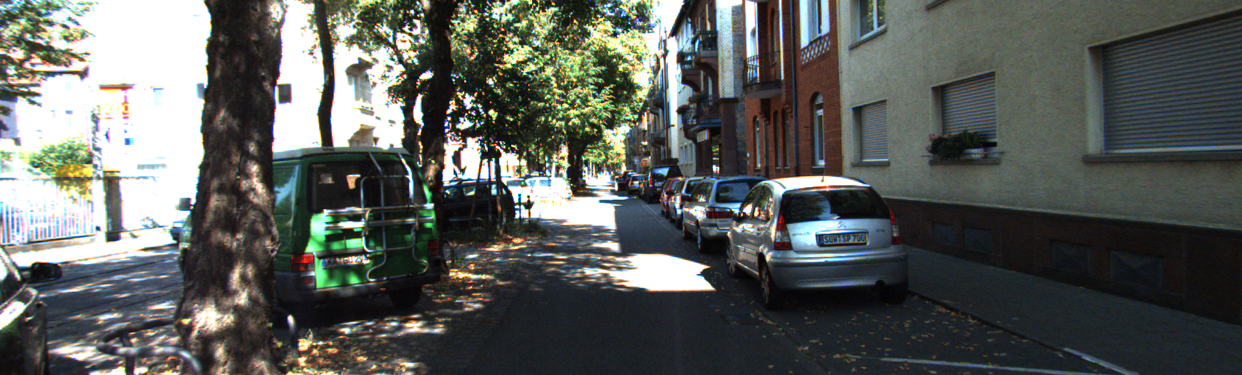
\includegraphics[width=0.45\textwidth]{figure/fig20.png}
    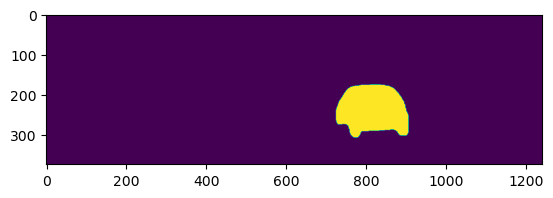
\includegraphics[width=0.45\textwidth]{figure/fig19.png}
    \caption{KITTI数据集的掩码标注}
    \label{fig19}
\end{figure}

由于我们希望较高的检测速度,以应对在线跟踪场景,且DAIR数据集不含掩码标注,不适合现有主流二阶段框架,我们选择了YOLO系列框架。为方便起见,我们采用了应用生态较为成熟的YOLOv4框架,没有使用最新的检测器。

\subsubsection{YOLOv4网络模型}

YOLOv4在YOLOv3的基础上,在数据增强、网络结构、网络训练方式、损失函数计算方式等方面进行改进。YOLOv4网络模型的主要贡献为:

\begin{enumerate}
    \item 提出了一种高效有力的目标检测模型,它可以使用一块1080Ti显卡或2080Ti显卡训练出快速且精确的目标检测器。
    \item 论文确认了检测器训练阶段,最先进的Bag of Specials和Bag of Freebies方法的效果。
    \item 论文修改了最先进的方法并且使它们在单GPU训练时更加高效合适,包括了CBN,PAN,SAM等
\end{enumerate}

其中,Bag of Freebies指不增加模型复杂度,也不增加推理的计算量的提高模型的准确度的训练方法技巧,Bag of Specials指增加少许模型复杂度或计算量,但可以显著提高模型的准确度的训练技巧。YOLOv4使用大量此类的技巧,提高了模型的性能。

目标检测器无论是一阶段还是二阶段,往往都可以划分为如图\ref{fig21}结构,由输入(Input),主干网络(Backbone),颈部网络(Neck),检测头(Head)与预测层(Prediction)组成。

\begin{figure}[htb] 
    \center
    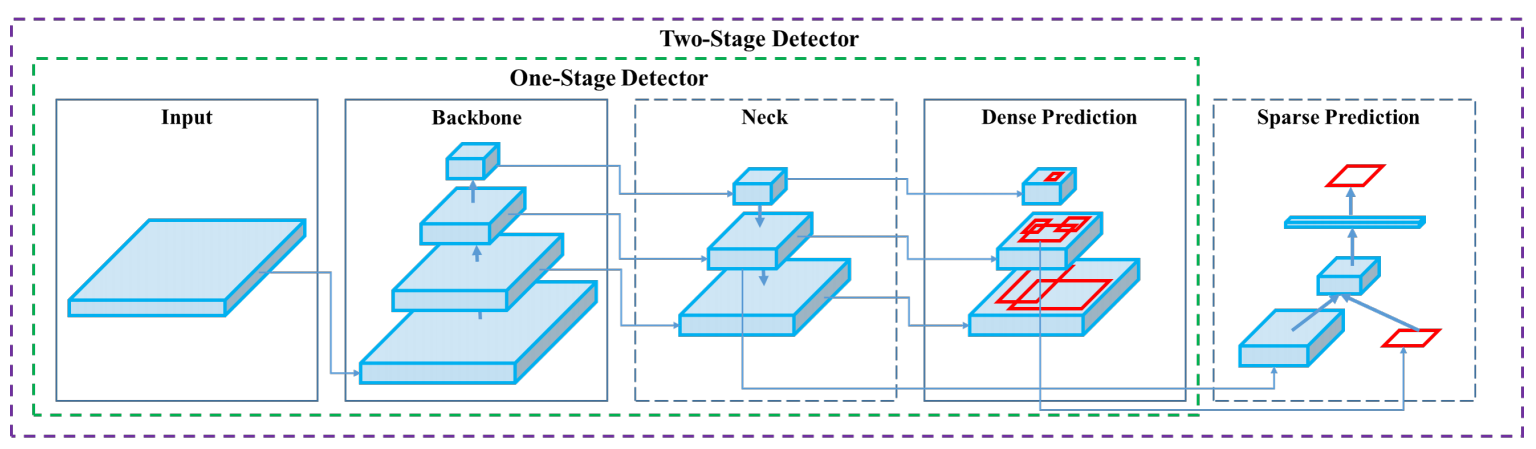
\includegraphics[width=\textwidth]{figure/fig21.png}
    \caption{目标检测框架流程图\cite{bochkovskiy2020yolov4}}
    \label{fig21}
\end{figure}

YOLOv4的网络结构如表\ref{table6}所示

\begin{table}[htbp]
    \centering
    \caption{YOLOv4网络模型}
    \begin{tabular}{c c}
    \toprule
    Module & Method \\
    \midrule
    Backbone & CSPDarknet53 \\
    Neck & SPP, PAN \\
    Head & YOLOv3 \\
    \bottomrule
    \end{tabular}
    \label{table6}
\end{table}

\textbf{输入层 Input}
YOLOv4网络模型在输入时进行了许多创新改进,例如Mosaic 数据增强、cmBN、SAT 自对抗训练等。

\textbf{主干网络 Backbone} 
YOLOv4采用的主干网络为 CSPDarknet53,CSPDarknet53是在Yolov3主干网络Darknet53的基础上,借鉴2019年CSPNet(Cross Stage Partial Network)的经验,产生的Backbone结构,其中包含了1个CBM和5个CSP模块。它解决了网络优化的梯度信息重复问题,既保证了推理速度和准确度,又减小了模型尺寸。YOLOv4还将DarknetConv2D的激活函数由LeakyReLU修改成了Mish。

\textbf{颈部网络 Neck} 
空间金字塔池化层SPP全称Spatial Pyramid Pooling,可以用来解决不同尺寸的特征图如何进入全连接层,增加主干网络的感受野,显著的分离最重要的上下文特征,补充语义信息。PAN(Path Aggregation Network)替代了YOLOv3的FPN(Feature Pyramid
Networks),加强了信息在特征金字塔中,自下而上的路径,提高了特征提取的能力。

\textbf{检测头 Head} 主体还是YOLOv3算法的检测头,但是把损失函数修改为了CIOU(Complete IoU)。CIOU将目标与anchor之间的距离,重叠率、尺度以及惩罚项都考虑进去,使得目标框回归变得更加稳定,不会像IoU和GIoU(Generalized IoU)一样出现训练过程中发散等问题。而惩罚因子把预测框长宽比拟合目标框的长宽比考虑进去。

\subsubsection{YOLOv4训练及结果}

YOLOv4有诸多复现版本,我们采用了AlexeyAB的版本在如表\ref{table7}所示的环境中对DAIR-V2X进行了训练。训练集由5042张图片构成,评测集由2016张图片构成。类别只有一种,即car。

\begin{table}[htb]
    \centering
    \caption{YOLOv4训练环境}
    \begin{tabular}{c c c c c c c}
    \toprule
    配置 & OS & GPU & CPU & CUDA & CUDNN & OpenCV \\
    \midrule
    版本 & \makecell{Windows\\10} & \makecell{Nvidia Geforce \\ RTX 2060m} & \makecell{R7\\ 4800H} & 12.1 & 8.x & 4.7\\
    \bottomrule
    \end{tabular}
    \label{table7}
\end{table}

训练时损失函数下降图如图\ref{fig23}所示。可以看出下降曲线相对平缓,在大约2000步迭代后已经趋于收敛。IOU阈值为50\%时,平均精度mAP(mean of Average Precision)达到了96.25\%以上。

\begin{figure}[htb] 
    \center
    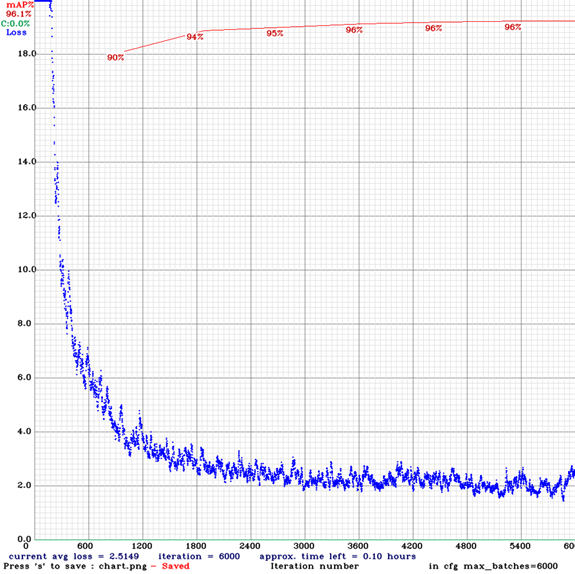
\includegraphics[width=0.6\textwidth]{figure/fig23.png}
    \caption{YOLOv4训练loss曲线}
    \label{fig23}
\end{figure}

评测结果如表\ref{table8}所示。
\begin{table}[htb]
    \centering
    \caption{YOLOv4测试结果}
    \begin{tabular}{c c c c c}
    \toprule
    检测器 & \makecell{精确率\\precison} & \makecell{召回率\\Recall} & mAP@0.5 & 平均IoU \\
    \midrule 
    YOLOv4 & 0.87 & 0.94 & 0.9625 & 0.77 \\
    \bottomrule
    \end{tabular}
    \label{table8}
\end{table}
其中,精确率定义为被正确预测的正样本数量占预测结果为正样本数量的比例,召回率定义为:被正确预测的正样本数量占真实结果为正样本数量的比例。目标检测过程中会生成大量预测框,每个预测框会有一个置信度属性。设置不同的置信度阈值,可以得到不同的输出。置信度越低,输出的预测框数量越大,召回率越高,但精确度越低,反之相反。如果设置不同的置信度阈值,就可以得到不同的召回率和准确率,将它们作为纵坐标与横坐标可以绘制一条曲线。曲线下方的区域面积定义为平均准确率AP(Average Precision)。所有类别的AP值的平均值定义为mAP。

如图\ref{fig24}为随机选取的几张图片的检测结果。
\begin{figure}[htb] 
    \center
    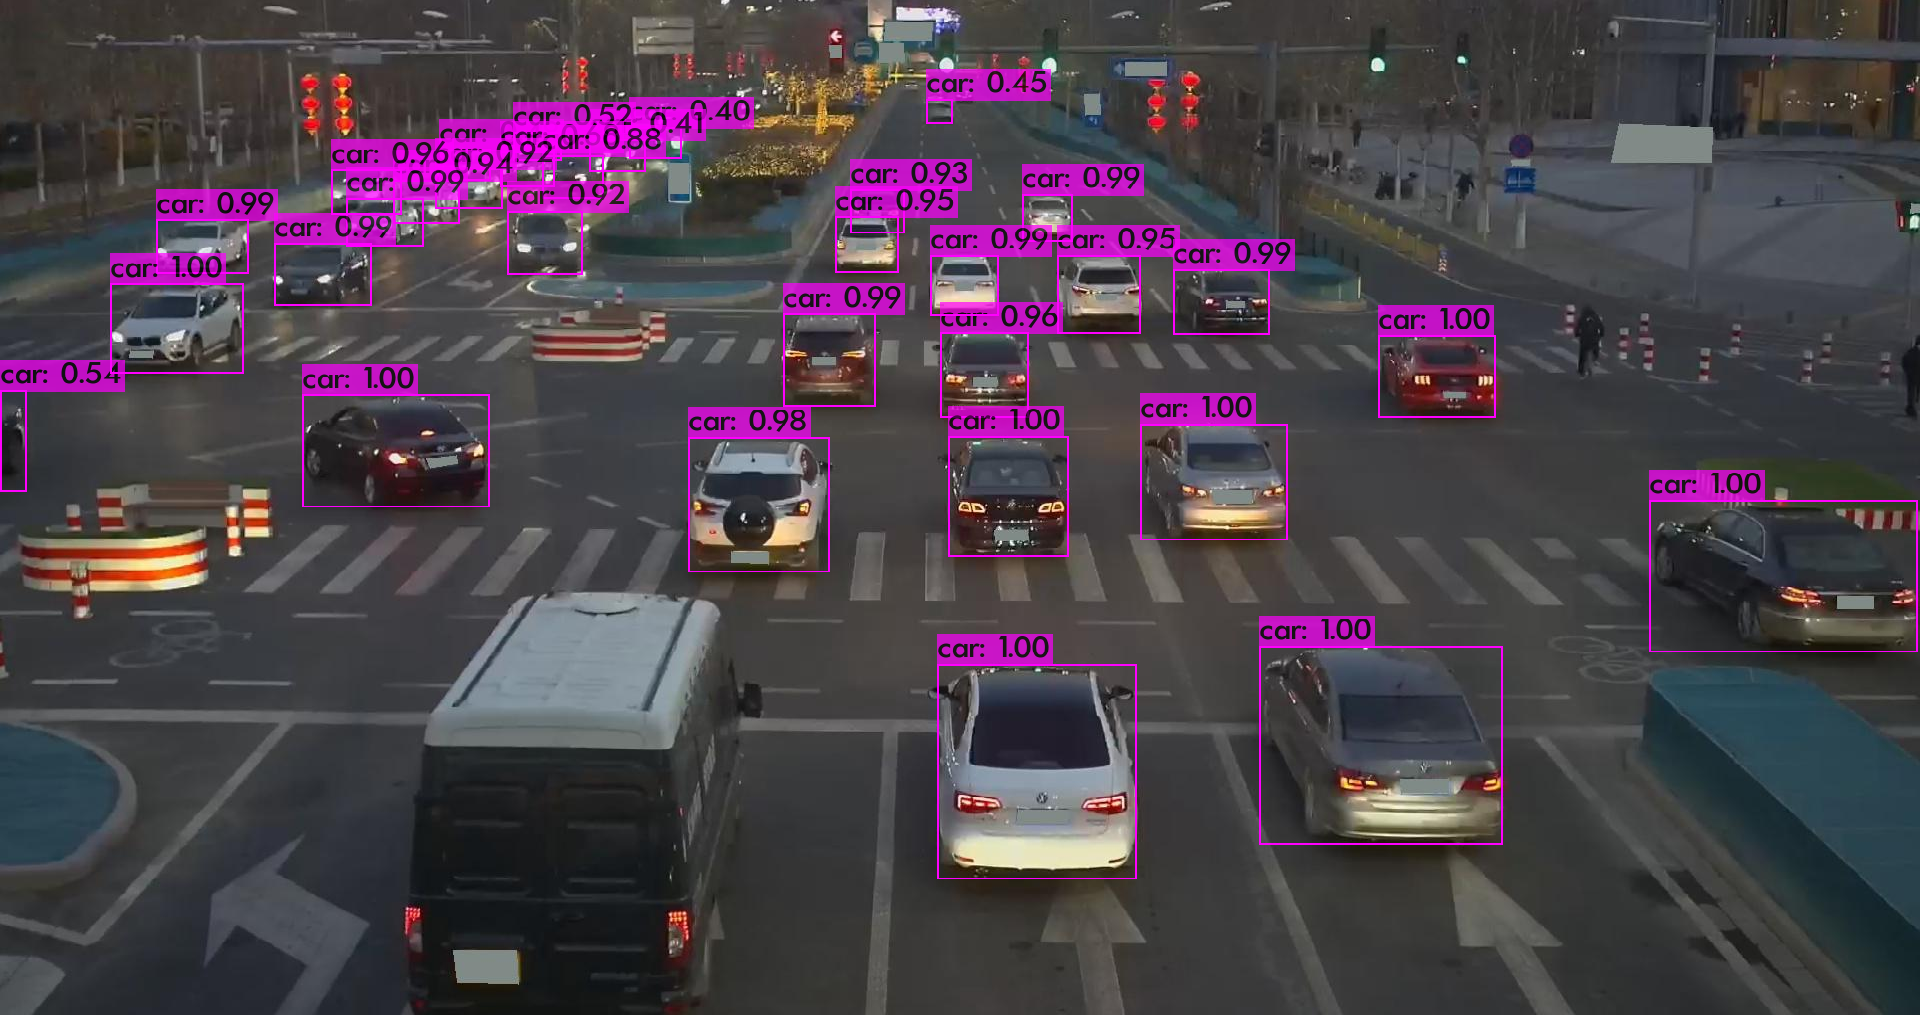
\includegraphics[width=0.45\textwidth]{figure/fig22.png}
    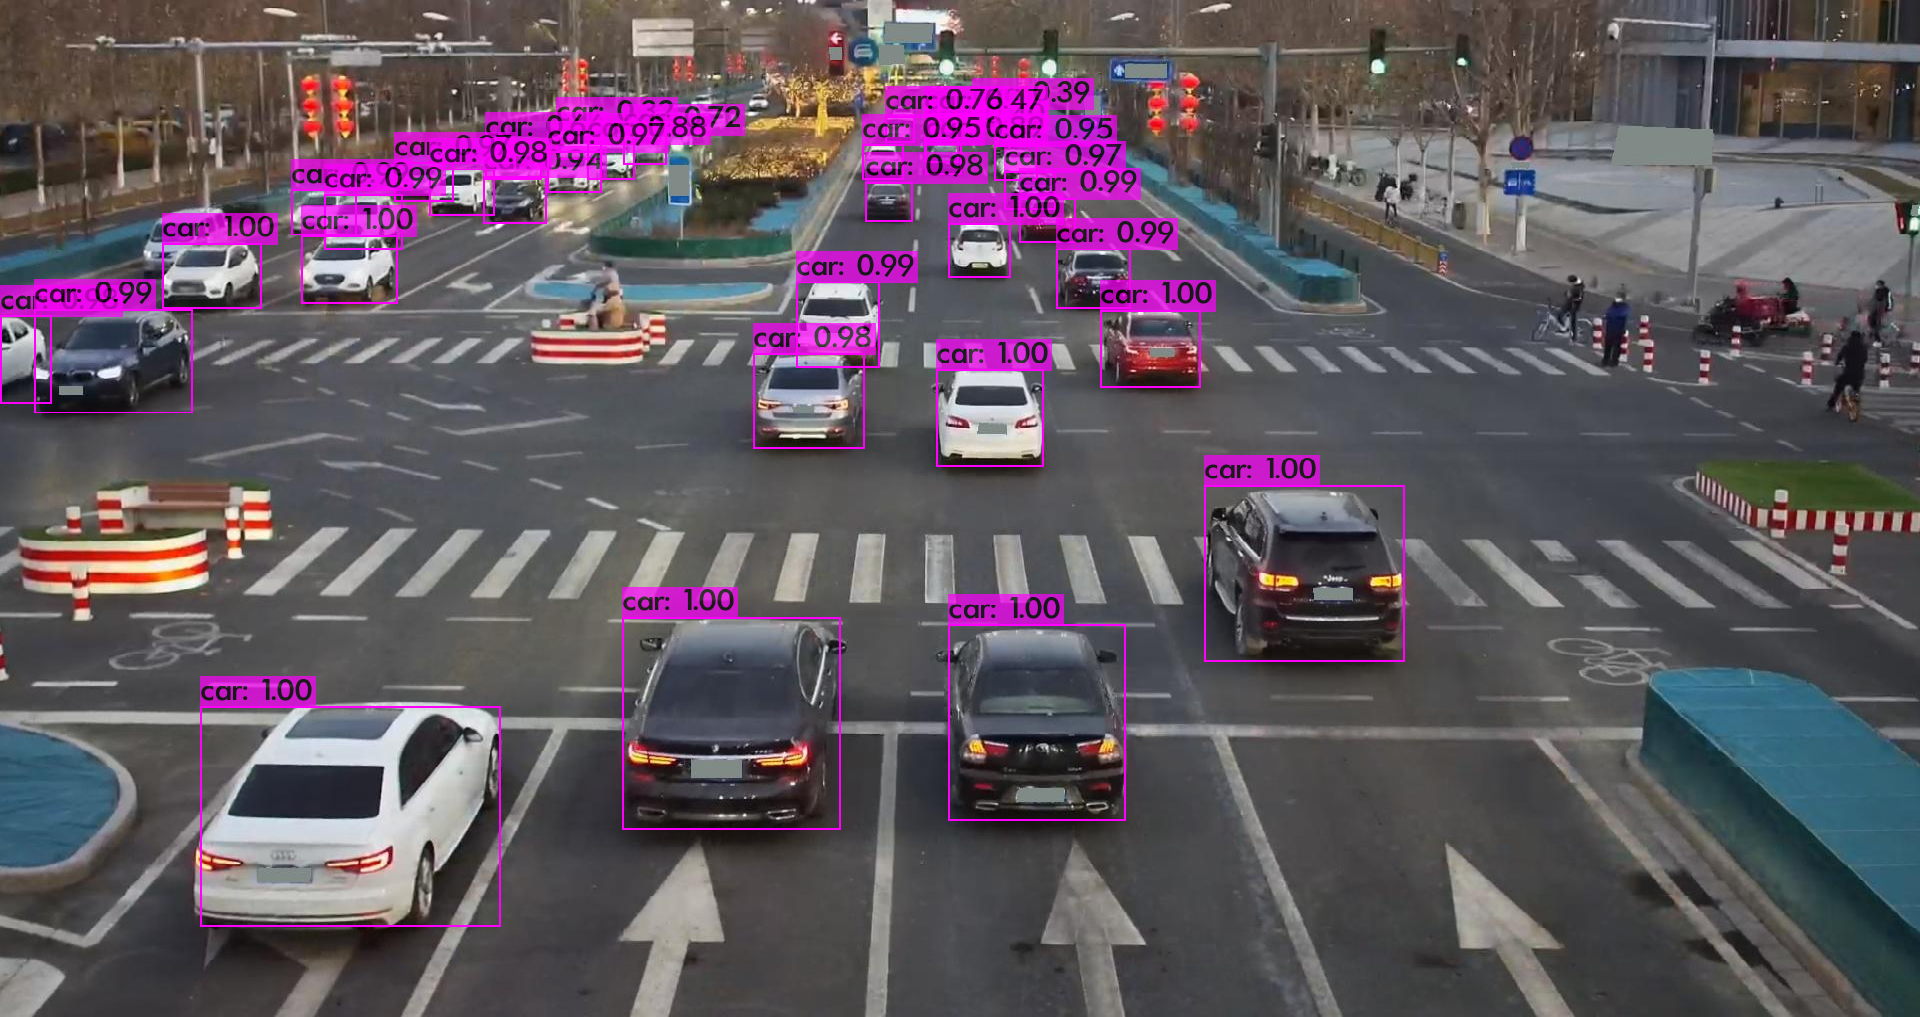
\includegraphics[width=0.45\textwidth]{figure/fig24.png}
    \caption{YOLOv4在评测集上的检测结果}
    \label{fig24}
\end{figure}
在制作标注文件时,我们没有将类型Van和Bus合并至类型Car中,因此部分大车型漏检严重,但常见的小轿车准确度较高。

\subsection{3D目标检测器}

\subsubsection{PointRCNN网络模型}

PointRCNN\cite{shi2019pointrcnn}是一个两阶段的点云目标检测算法,其可以直接对原始点云数据进行目标检测,无需对其投影至某一视角或对其体素化。该算法分为两大阶段:(1)基于点云分割的提议区域生成(2)标准坐标系下的边界框优化。整体示意图如图所示

\begin{figure}[htb] 
    \center
    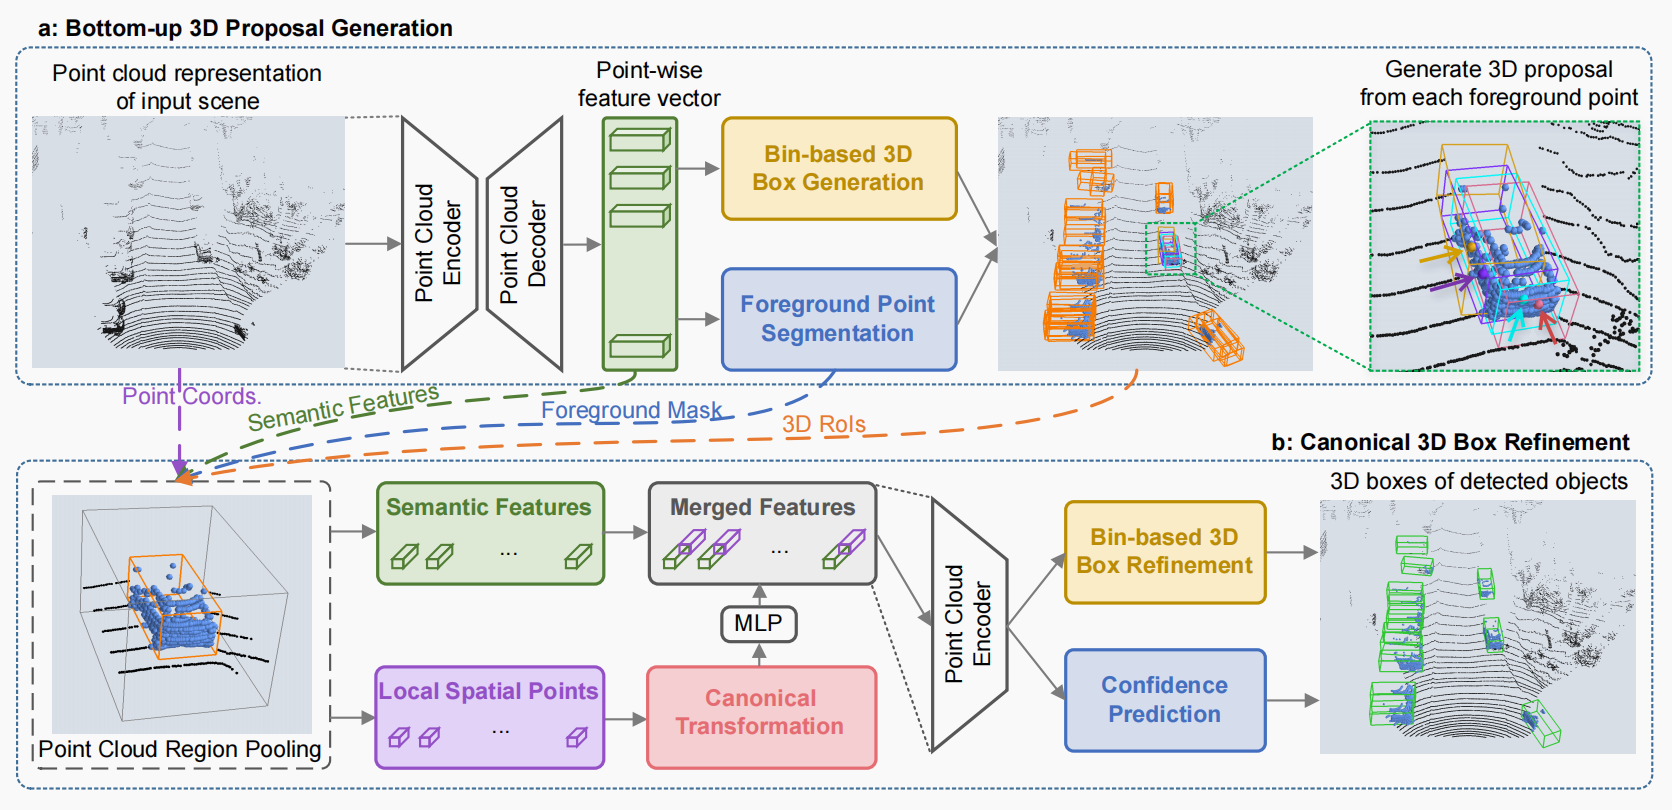
\includegraphics[width=0.9\textwidth]{figure/fig27.png}
    \caption{PointRCNN网络模型示意图\cite{shi2019pointrcnn}}
    \label{fig27}
\end{figure}

\textbf{第一阶段:基于点云分割的提议区域生成}

首先,为了获得原始点云的逐点判别特征,算法采用了PointNet++\cite{qi2017pointnet++}作为骨干网络。其中,其他的网络也可以替代这个位置,例如VoxelNet\cite{zhou2018voxelnet}等。

其次,算法对点云进行了前景点云分割处理。前景点提供了预测目标位置和方向的丰富信息。通过学习分割前景点,点云网络捕获了上下文信息以进行准确的逐点预测,这也有利于 3D 边界框生成。

最后,算法还添加了一个边界框回归头,用来同步地生成3D提议区域。为了约束生成的3D边界框,相对精准地预测目标的位置信息,每个前景点的周围区域,被沿着$X$轴与$Y$轴划分为了一系列离散的"bins"。算法对前景点的$X$轴与$Y$轴设置了一个搜索范围$S$,每个范围都被划分为了长宽均为$\delta$的bins,从而表示不同的目标中心坐标$(x,z)$。

\textbf{点云池化处理}

在获得第一阶段生成的㕺框后,算法对预选框进行了逐点池化处理,通过分割掩码,进行预选框内部前景点与背景点的分类。其中不包含点的预选框会被清除。

\textbf{第二阶段:标准坐标系下的边界框优化}

首先算法将池化后的点的坐标通过正规坐标变换,变换到标准坐标系,使得(1)坐标原点位于边界框中心,(2)坐标系的$X-Y$平面与地面平行,且$X$轴与边界框朝向一致,(3)$Y$轴与激光雷达坐标系的$Y$轴一致。

然后,算法学习了预选框优化特征。并增加了深度信息$$d^{(p)}=\sqrt{(x^{(p)})^2+(y^{(p)})^2+(z^{(p)})^2}$$以补偿坐标变化下的位置信息损失。在对预选框优化时,算法采用了如下的损失函数,完成回归。

\begin{equation}
    \begin{aligned}
        \mathcal{L}_{\text {refine }}= & \frac{1}{\|\mathcal{B}\|} \sum_{i \in \mathcal{B}} \mathcal{F}_{\mathrm{cls}}\left(\operatorname{prob}_{i}, \text { label }_{i}\right) \\
        & +\frac{1}{\left\|\mathcal{B}_{\text {pos }}\right\|} \sum_{i \in \mathcal{B}_{\text {pos }}}\left(\tilde{\mathcal{L}}_{\text {bin }}^{(i)}+\tilde{\mathcal{L}}_{\text {res }}^{(i)}\right)
        \end{aligned}
\end{equation}

\subsubsection{PointRCNN训练及结果}

我们在DAIR-V2X数据集上应用了PointRCNN算法。设置batchsize为4,epoch为200,训练了RPN网络,设置batchsize为2,epoch为70,训练了RCNN网络。然后在评测集上进行了测试,实验结果如表\ref{table9}所示。

\begin{table}[htb]
    \centering
    \caption{PointRCNN测试结果}
    \begin{tabular}{c c c c c c}
    \toprule
    难度 & bbox & bev & 3d & aos \\
    \midrule 
    简单(Easy) & 81.5738 & 80.1970 & 69.2464 & 77.56 \\
    中等(Moderate) & 80.4673 & 78.2905 & 65.6314 & 76.28 \\
    困难(Hard) & 79.4982 & 78.2205 & 65.5195 & 77.14 \\
    \bottomrule
    \end{tabular}
    \label{table9}
\end{table}
其中难度是数据集根据车辆被遮挡,截断的程度设置的检测难易程度。bbox是指2D检测框的准确度,bev指鸟瞰图下的检测框准确度,3d为3D检测框的准确度,aos为检测目标的旋转角的准确度。值得注意的是,表\ref{table9}中所有结果均是IoU为0.7的设置下得到的。

如图\ref{fig26}所示为序列000018的检测结果。其中左图为点云可视化结果,红色边界框为标注数据,即真值,蓝色边界框为预测结果。右图为标注信息投影至图像中的结果,不包含目标检测结果。检测框架仅对图像中出现的车辆进行检测,由于第二章所述坐标系变换的原因,部分距离较近的车辆没有被识别。远处的车辆,被遮挡严重的没有被识别。在中等距离下的识别效果较好。值得注意的是,数据集本身的标注质量较为一般,例如图中最靠近观察点的三辆车,即图片最下方的3个车辆,标注的车辆高度明显比车辆的实际高度要小,车辆的车顶甚至比标注的边界框高出了不少。但我们识别出的车辆边界框还是比较符合现实的,比标注的要大一些。

\begin{figure}[htb] 
    \center
    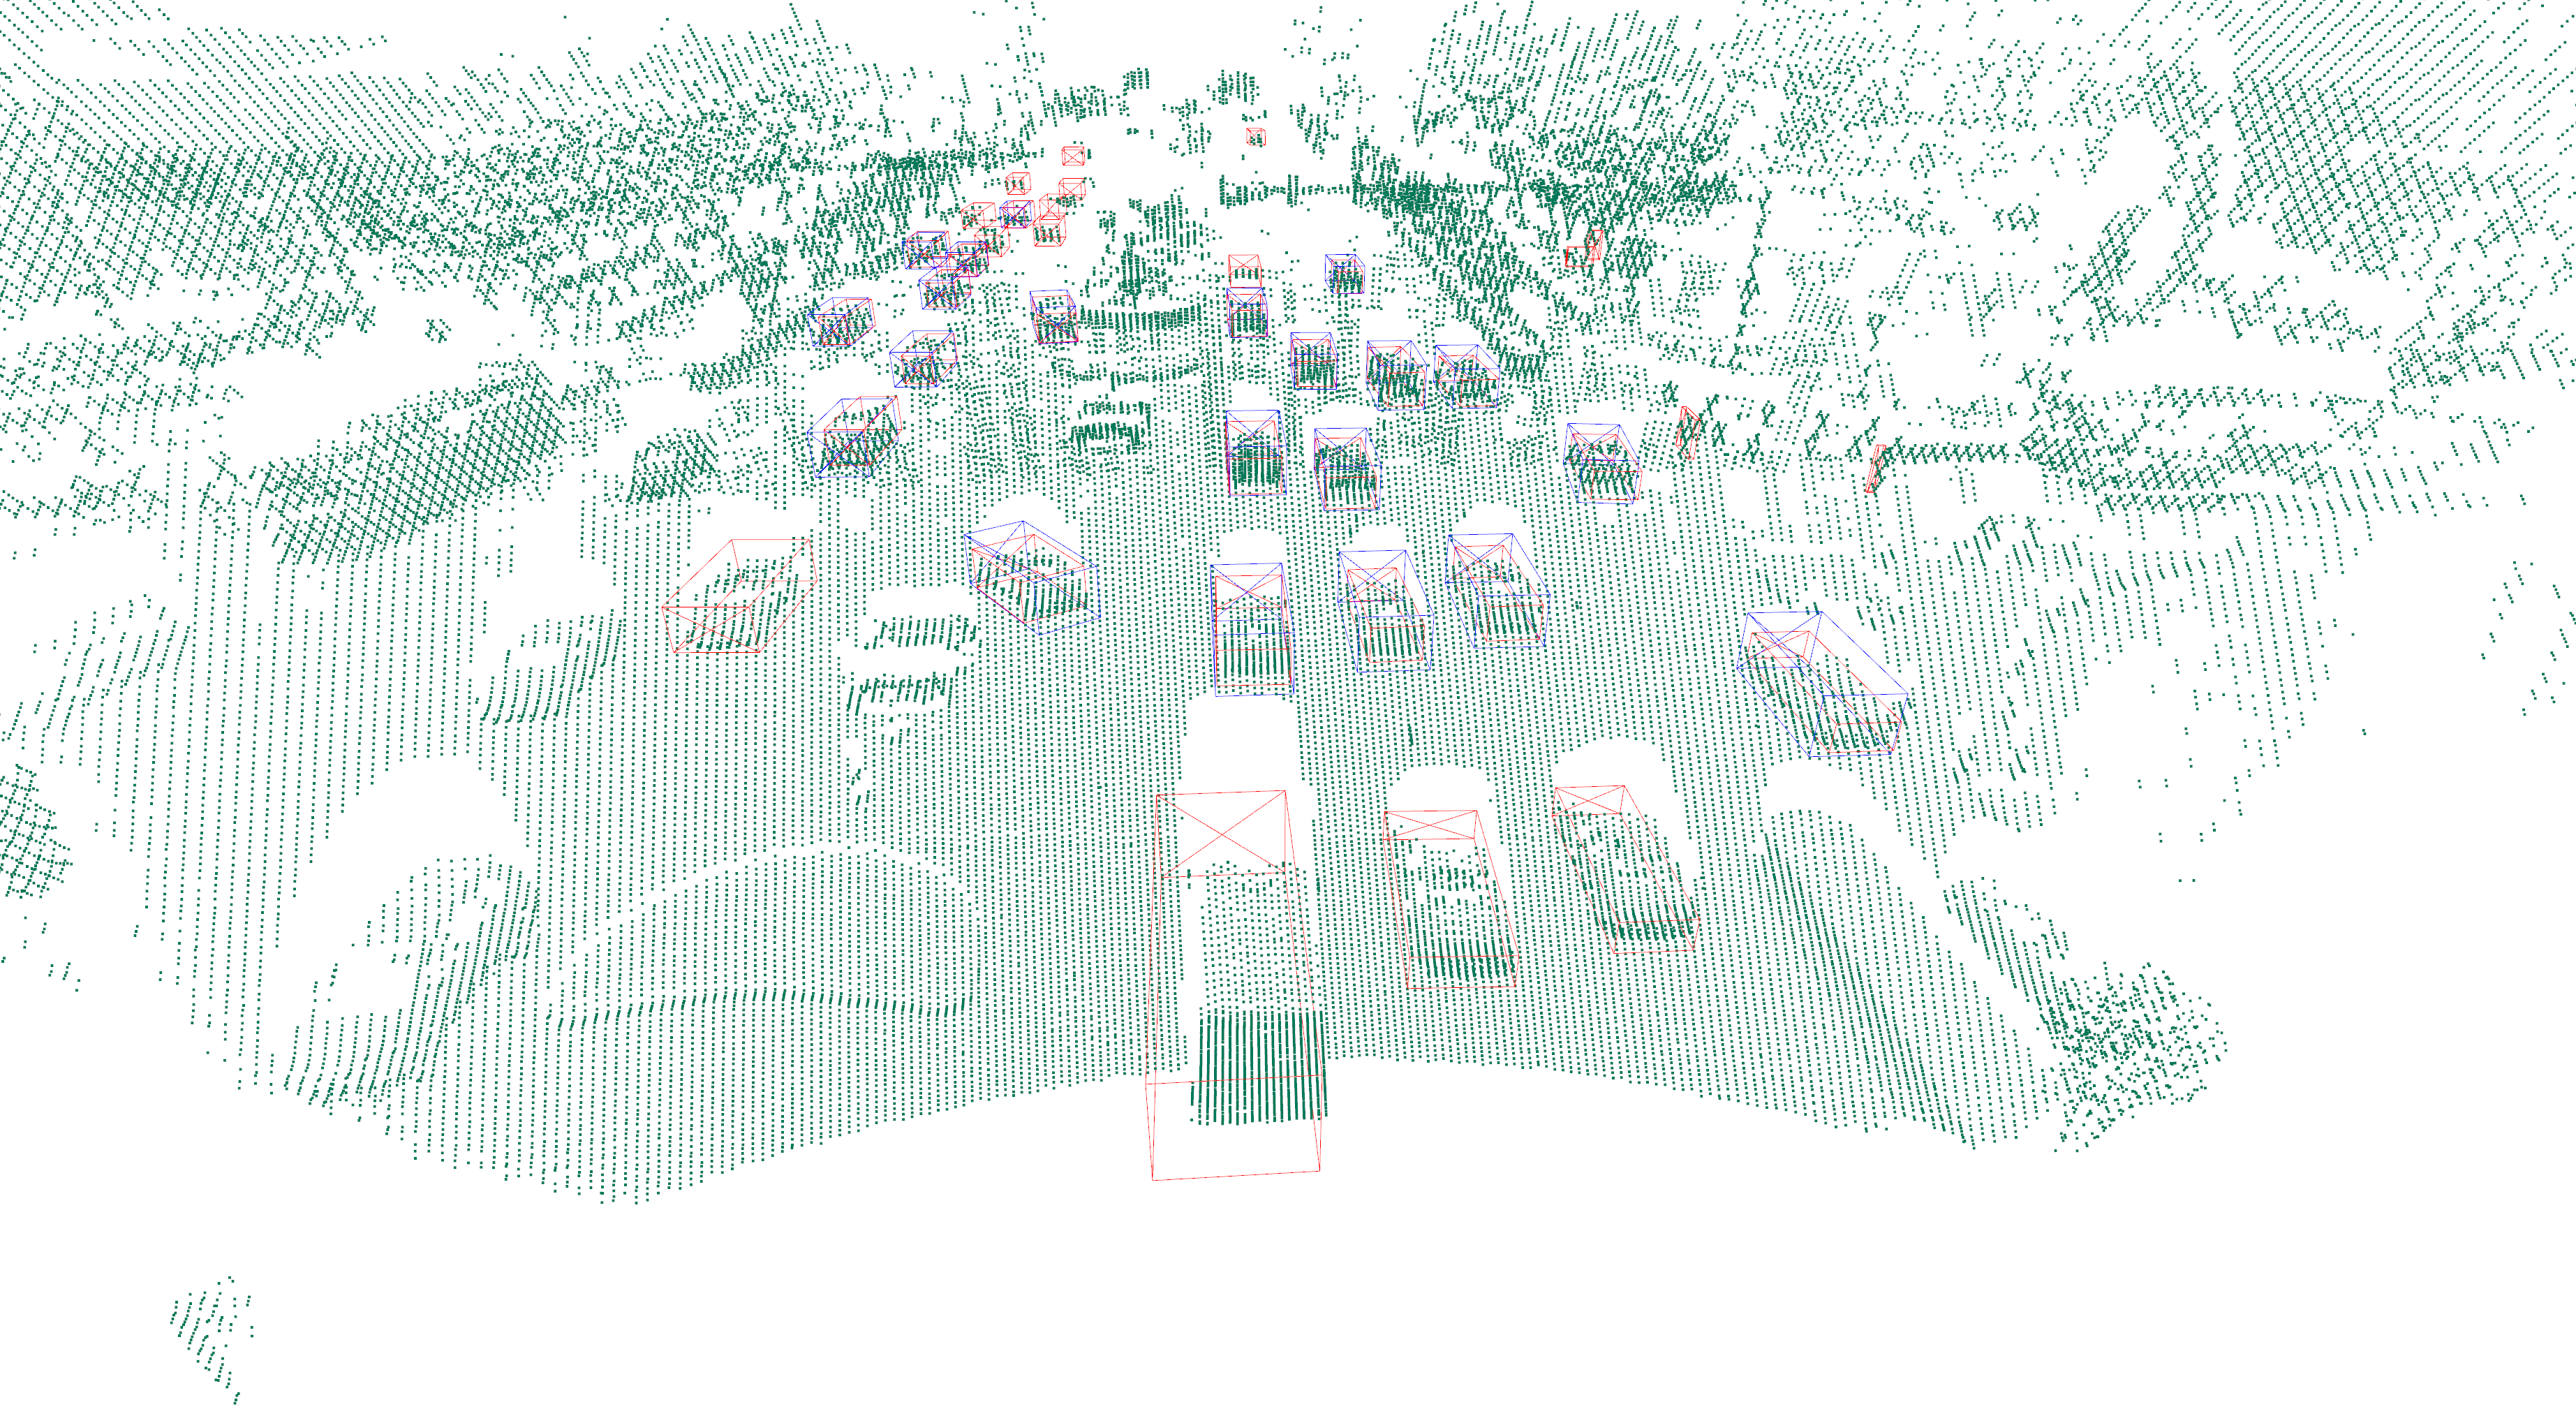
\includegraphics[width=0.48\textwidth]{figure/fig26.png}
    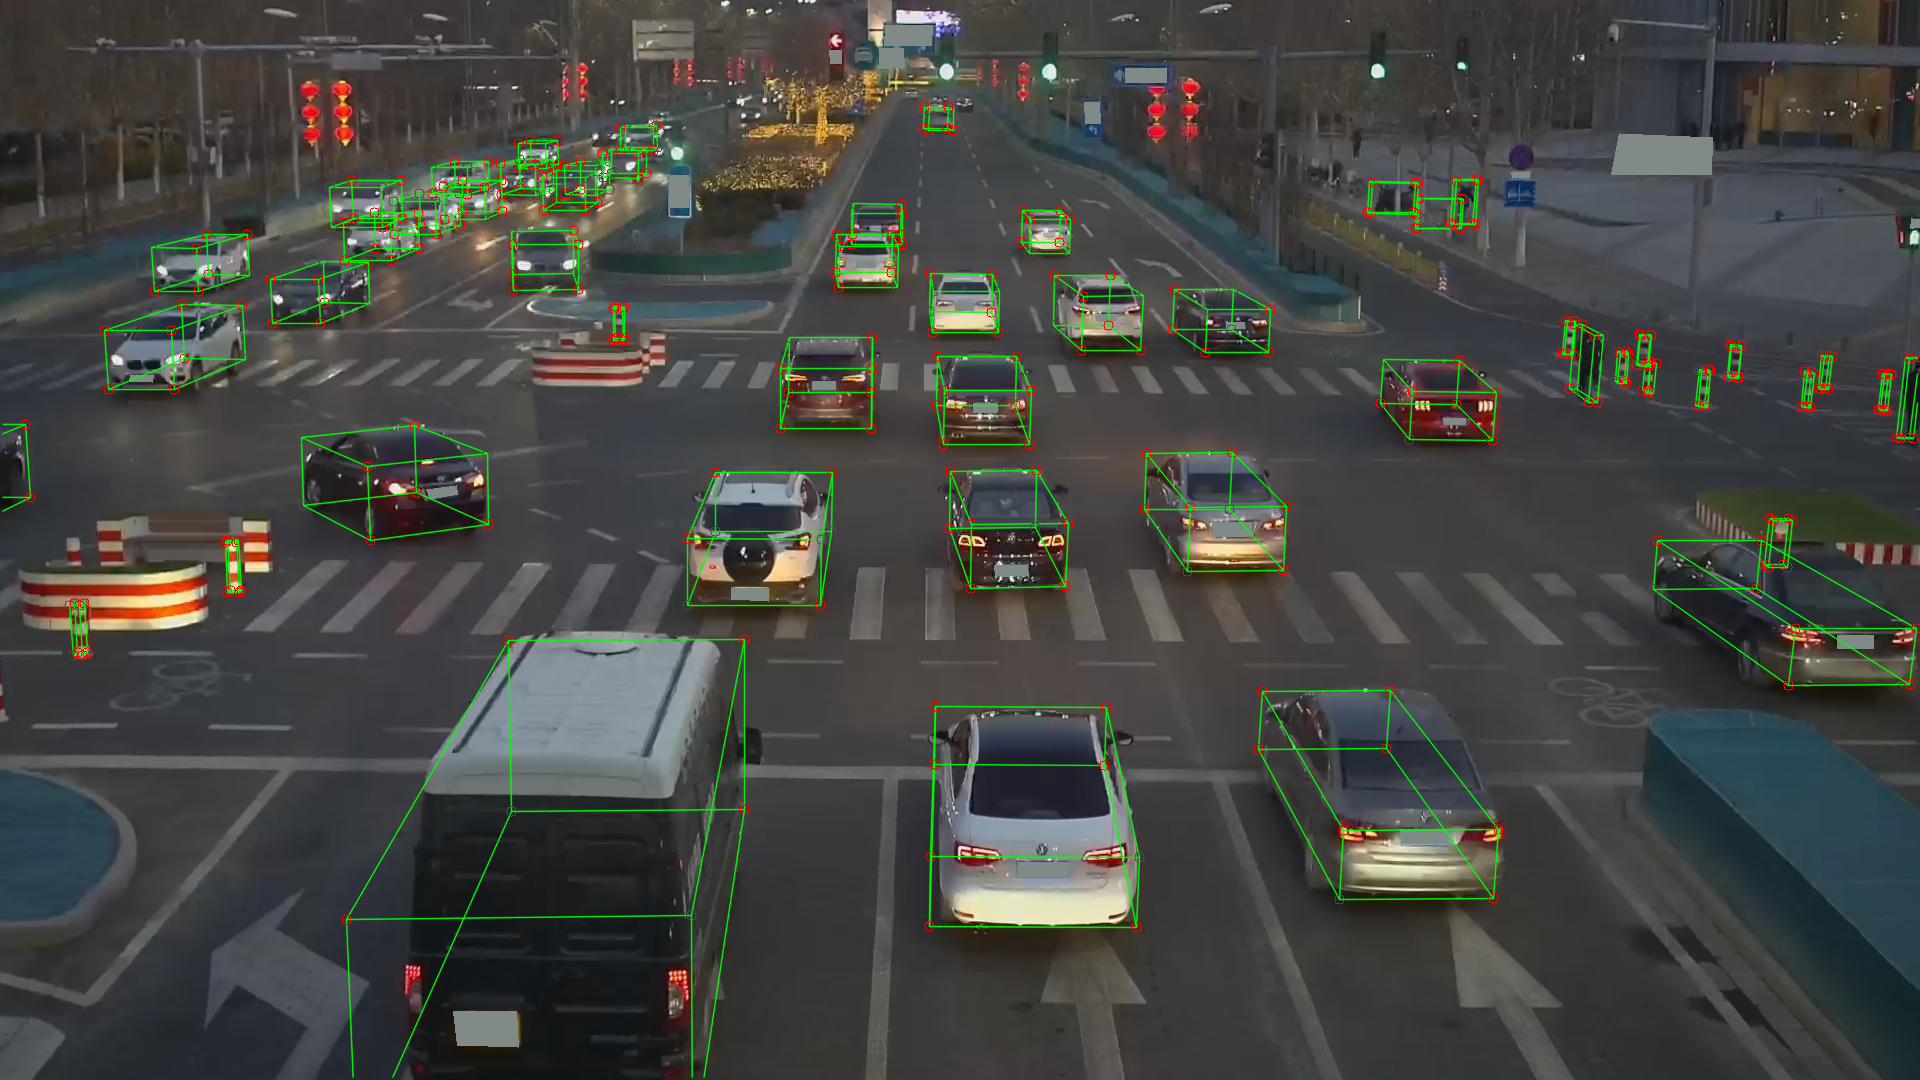
\includegraphics[width=0.48\textwidth]{figure/fig9.png}
    \caption{DAIR-V2X序列000018的检测结果}
    \label{fig26}
\end{figure}

\subsection{本章小结}

本章首先介绍了2D检测器YOLOv4的原理,训练环境与网络配置,训练结果,结果分析。再介绍了3D检测器PointRCNN的原理,训练环境与网络配置,训练结果,结果分析。